%%%%%%%%%%%%%%%%%%%%%%%%%%%%%%%%%%%%%%%
% Wenneker Resume/CV
% LaTeX Template
% Version 1.1 (19/6/2016)
%
% This template has been downloaded from:
% http://www.LaTeXTemplates.com
%
% Original author:
% Frits Wenneker (http://www.howtotex.com) with extensive modifications by 
% Vel (vel@LaTeXTemplates.com) and Alexey Ermolenko (ermolenkoav@gmail.com)
%
% License:
% CC BY-NC-SA 3.0 (http://creativecommons.org/licenses/by-nc-sa/3.0/
%
%%%%%%%%%%%%%%%%%%%%%%%%%%%%%%%%%%%%%%

\documentclass[a4paper,12pt]{memoir} % Font and paper size
%%%%%%%%%%%%%%%%%%%%%%%%%%%%%%%%%%%%%%%%%
% Wenneker Resume/CV
% Structure Specification File
% Version 1.1 (19/6/2016)
%
% This file has been downloaded from:
% http://www.LaTeXTemplates.com
%
% Original author:
% Frits Wenneker (http://www.howtotex.com) with extensive modifications by 
% Vel (vel@latextemplates.com)
%
% License:
% CC BY-NC-SA 3.0 (http://creativecommons.org/licenses/by-nc-sa/3.0/)
%
%%%%%%%%%%%%%%%%%%%%%%%%%%%%%%%%%%%%%%%%%

%----------------------------------------------------------------------------------------
%	PACKAGES AND OTHER DOCUMENT CONFIGURATIONS
%----------------------------------------------------------------------------------------

\usepackage{XCharter} % Use the Bitstream Charter font
\usepackage[utf8]{inputenc} % Required for inputting international characters
\usepackage[T1]{fontenc} % Output font encoding for international characters

\usepackage[top=1cm,left=1cm,right=1cm,bottom=1cm]{geometry} % Modify margins

\usepackage{graphicx} % Required for figures

\usepackage{flowfram} % Required for the multi-column layout

\usepackage{hyperref} % URLs
\hypersetup{colorlinks=true,linkcolor=blue,urlcolor=blue}
\urlstyle{rm}

\usepackage[usenames,dvipsnames]{xcolor} % Required for custom colours

\usepackage{tikz} % Required for the horizontal rule

\usepackage{enumitem} % Required for modifying lists
\setlist{noitemsep,nolistsep} % Remove spacing within and around lists

\setlength{\columnsep}{\baselineskip} % Set the spacing between columns

% Define the left frame (sidebar)
\newflowframe{0.2\textwidth}{\textheight}{0pt}{0pt}[left]
\newlength{\LeftMainSep}
\setlength{\LeftMainSep}{0.2\textwidth}
\addtolength{\LeftMainSep}{1\columnsep}
 
% Small static frame for the vertical line
\newstaticframe{1.5pt}{\textheight}{\LeftMainSep}{0pt}
 
% Content of the static frame with the vertical line
\begin{staticcontents}{1}
\hfill
\tikz{\draw[loosely dotted,color=RoyalBlue,line width=1.5pt,yshift=0](0,0) -- (0,\textheight);}
\hfill\mbox{}
\end{staticcontents}
 
% Define the right frame (main body)
\addtolength{\LeftMainSep}{1.5pt}
\addtolength{\LeftMainSep}{1\columnsep}
\newflowframe{0.7\textwidth}{\textheight}{\LeftMainSep}{0pt}[main01]

\pagestyle{empty} % Disable all page numbering

\setlength{\parindent}{0pt} % Stop paragraph indentation

%----------------------------------------------------------------------------------------
%	NEW COMMANDS
%----------------------------------------------------------------------------------------

\newcommand{\userinformation}[1]{\renewcommand{\userinformation}{#1}} % Define a new command for the CV user's information that goes into the left column

\newcommand{\cvheading}[1]{{\Huge\bfseries\color{RoyalBlue} #1} \par\vspace{.6\baselineskip}} % New command for the CV heading
\newcommand{\cvsubheading}[1]{{\Large\bfseries #1} \bigbreak} % New command for the CV subheading

\newcommand{\Sep}{\vspace{1em}} % New command for the spacing between headings
\newcommand{\SmallSep}{\vspace{0.5em}} % New command for the spacing within headings

\newcommand{\aboutme}[2]{ % New command for the about me section
\textbf{\color{RoyalBlue} #1}~~#2\par\Sep
}
	
\newcommand{\CVSection}[1]{ % New command for the headings within sections
{\Large\textbf{#1}}\par
\SmallSep % Used for spacing
}

\newcommand{\CVItem}[2]{ % New command for the item descriptions
\textbf{\color{RoyalBlue} #1}\par
#2
\SmallSep % Used for spacing
}

\newcommand{\bluebullet}{\textcolor{RoyalBlue}{$\circ$}~~} % New command for the blue bullets
 % Include the file specifying document layout and packages

\userinformation{ % Set the content that goes into the sidebar of each page
\begin{flushright}
% Comment out this figure block if you don't want a photo
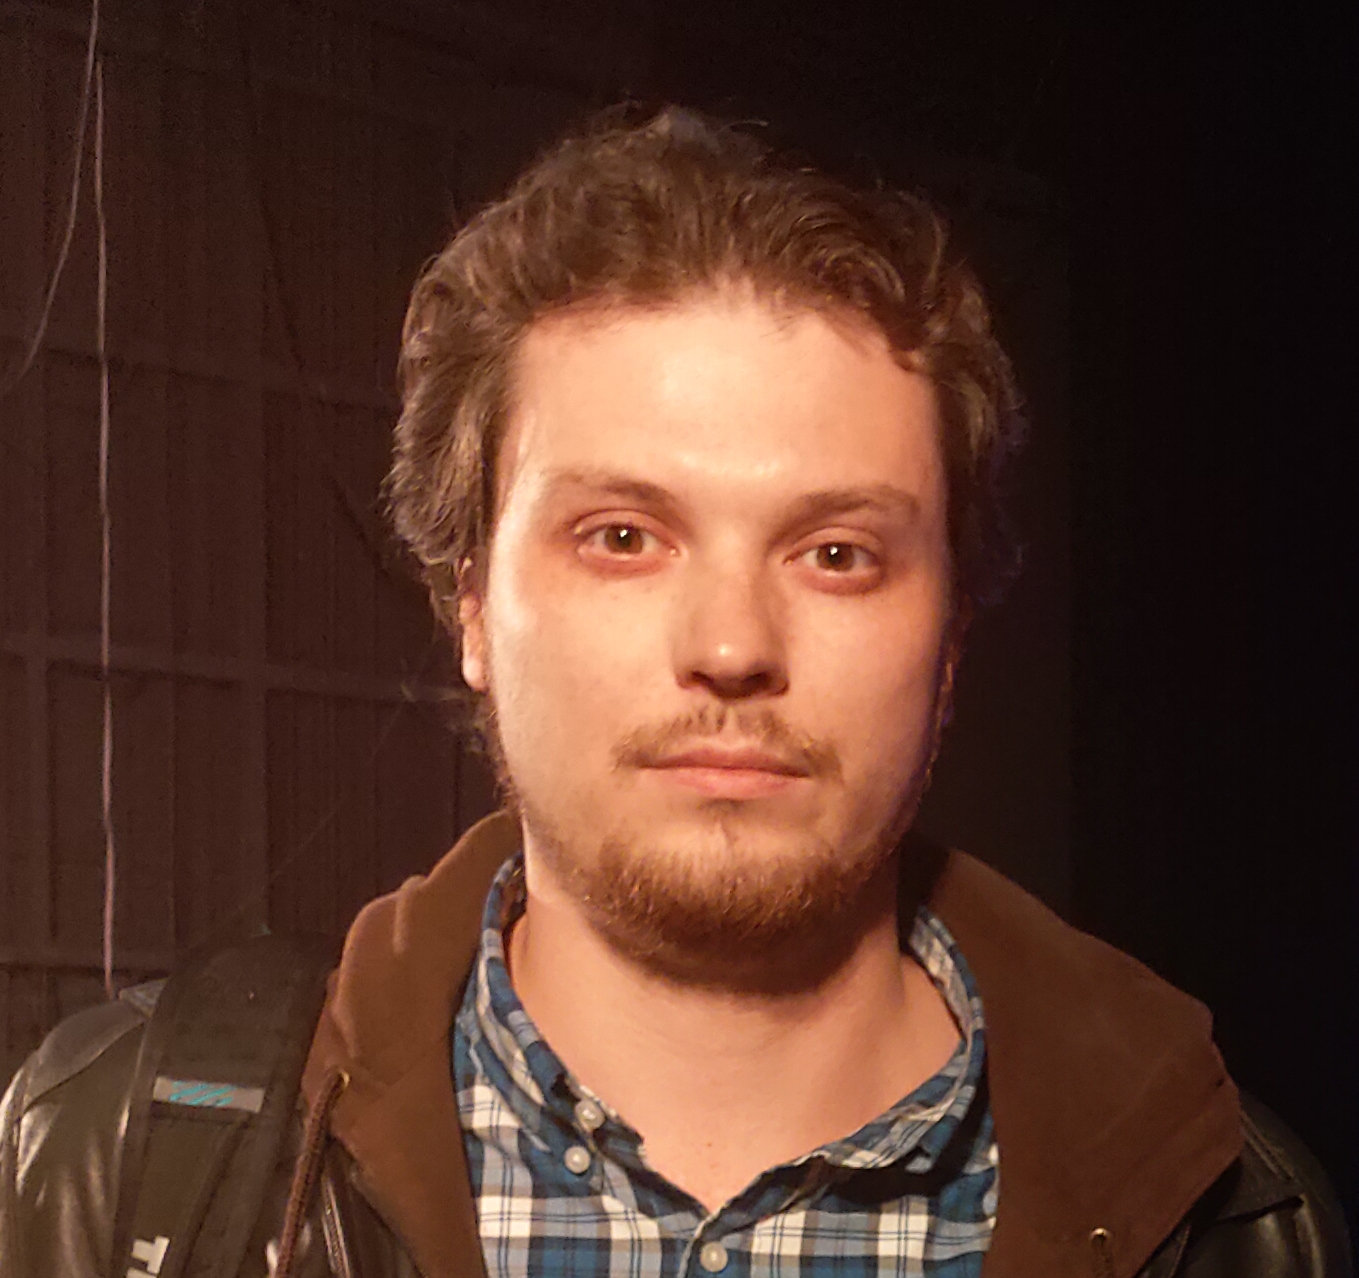
\includegraphics[width=1\columnwidth]{photo}\\[\baselineskip] % Your photo
\small % Smaller font size
\textbf{Contacts} \\ % Name
\href{https://ermolenkoav.t.me/}{Telegram} \\ % Email
\href{https://www.linkedin.com/in/ermolenkoav/}{LinkedIn} \\ % Your URL
\href{https://github.com/ermolenkoav}{GitHub} \\
\href{mailto:ermolenkoav@gmail.com}{Email} \\ % Email
+7 (918) 565--36--01 \\ % Your phone number
\Sep % Some whitespace
\textbf{Address} \\
Rostov-on-Don, Russia \\ 
\vfill % Whitespace under this block to push it up under the photo
\end{flushright}
}

%----------------------------------------------------------------------------------------
\begin{document}
\userinformation % Print your information in the left column
\framebreak % End of the first column

%----------------------------------------------------------------------------------------
%	HEADING
%----------------------------------------------------------------------------------------

\cvheading{Alexey Ermolenko}
\cvsubheading{Software Engineer}

%----------------------------------------------------------------------------------------
%	ABOUT ME
%----------------------------------------------------------------------------------------

\aboutme{About Me}{Actively participated in all stages of life cycle development of software and hardware for big data collection and processing. Including: development of highload back-end microservices, SQL and NoSQL database structure design, client-server and embedded software by the client's order, implementation of the maximum number of functionalities with limited computing resources, support and refactoring of third-party and company's legacy software, introduction of new technologies and approaches. Wrote design and supporting development documentation. Participated in presentation events: \href{https://youtu.be/1QDFi3-sKCY}{Living Sensors}}

%----------------------------------------------------------------------------------------
%	SKILLS
%----------------------------------------------------------------------------------------

\CVSection{Software Development Skills}

\CVItem{Programming}
{\begin{tabular}{ l l l l l }
\bluebullet Golang & \bluebullet SQL & \bluebullet C/C++ & \bluebullet Python & \bluebullet Java \\
\end{tabular}}

\CVItem{Computer Software}
{\begin{tabular}{ l l l }
\bluebullet Docker & \bluebullet Docker Compose & \bluebullet K8s \\
\end{tabular}}

%----------------------------------------------------------------------------------------
%	EXPERIENCE
%----------------------------------------------------------------------------------------

\CVSection{Experience}

\CVItem{October 2022 - Now, \textit{Software Engineer}, WB Tech ltd.}{
\begin{itemize}
    \item Create ClickHouse databases design and implemented for real-time display of financial metrics
	\item Replaced the NATS cluster with the Kafka cluster of all user-balance department services
	\item Development of integration services 
	\begin{itemize}
		\item Golang - fasthttp,pgx,clickhouse-go e.t.c
	\end{itemize}
	\item Developed database design and implemented a financial analytics system
	\begin{itemize}
		\item ClickHouse NoSQL
	\end{itemize}
\end{itemize}
}

\CVItem{October 2021 - June 2022, \textit{Software Engineer}, DDoS-Guard ltd.}{
\begin{itemize}
	\item Working with highload proxy server - implementation of new functionality and refactoring 
	\begin{itemize}
		\item C++ - STL, Boost, GoogleTest
	\end{itemize}
	\item Participated in the development of  of l4 load balancer
	\begin{itemize}
		\item Linux/eBPF, Golang/\href{https://github.com/cilium/ebpf}{Cilium eBPF}
	\end{itemize}
	\item Writing technical documentation
	\begin{itemize}
		\item \href{Diagrams.net}{Draw.io}, \LaTeX{}, 
	\end{itemize}
\end{itemize}
}

\CVItem{February 2020 - October 2021, \textit{Software Engineer}, Rostpay ltd.}{
\begin{itemize}
	\item Development client-server desktop application
	\begin{itemize}
		\item C++, STL, \href{https://github.com/pocoproject/poco}{POCO Libraries}, wxWidgets, GoogleTest, Win32, Design patterns
	\end{itemize}
	\item Customize Chromium browser
	\begin{itemize}
		\item C++ - STL, Chromium, Working inside a large volume of code
	\end{itemize}
	\item Writing support and technical documentation
	\begin{itemize}
		\item \href{Diagrams.net}{Draw.io}
	\end{itemize}
\end{itemize}
}

%----------------------------------------------------------------------------------------
%	NEW PAGE DELIMITER
%	Place this block wherever you would like the content of your CV to go onto the next page
%----------------------------------------------------------------------------------------

\clearpage % Start a new page

\userinformation % Print your information in the left column

\framebreak % End of the first column

%----------------------------------------------------------------------------------------

\CVItem{November 2017 - January 2020, \textit{Software Engineer}, R\&D Center for Neurotechnology, SFedU.}{
\begin{itemize}
	\item Development of client programs to control the experiment using
	\begin{itemize}
		\item C/C++ - STL, Qt Widgets, Boost, GoogleTest, Win32
	\end{itemize}
	\item Development of electronic devices and software based on technology
	\begin{itemize}
		\item Texas Instruments CC2541,CC2540, Altium Designer, Atmel AVR
	\end{itemize}
	\item Writing support and technical documentation
	\item Assembly and maintenance of electronic devices
\end{itemize}
}

\CVItem{Febrary 2015 - October 2017, \textit{Software Engineer}, Don-Strike ltd.}{
\begin{itemize}
	\item Development of electronic devices and software based on technology
	\begin{itemize}
		\item C/C++ - STL, Qt
		\item Texas Instruments CC2541,CC2540, Altium Designer, Atmel AVR
	\end{itemize}
	\item Writing support and technical documentation
	\begin{itemize}
		\item \LaTeX{}
	\end{itemize}
	\item Assembly and maintenance of electronic devices
\end{itemize}
}

\CVItem{September 2013 - Febrary 2015, \textit{Junior Software Engineer}, FGANU Research Institute Spetsvuzavtomatika.}{
\begin{itemize}
	\item Participation in the development of electronic devices
	\begin{itemize}
		\item Atmel AVR, Atmel Designer
	\end{itemize}
	\item Prototyping electronic circuits
\end{itemize}
}

\tiny

%----------------------------------------------------------------------------------------
%	EDUCATION
%----------------------------------------------------------------------------------------
\CVSection{Education}
\CVItem{2011 - 2014, Southern Federal University}{Department of Physics, Postgraduate School}

\CVItem{2006 - 2011, Southern Federal University}{Department of Physics, Medical Physics}
\Sep % Extra whitespace after the end of a section

%----------------------------------------------------------------------------------------
%	LANGUAGE SKILLS
%----------------------------------------------------------------------------------------
\CVSection{Language skills}
\CVItem{Russian}{Native}

\CVItem{English}{B1 Strong Pre-Intermediate}
\Sep % Extra whitespace after the end of a section

%----------------------------------------------------------------------------------------
%	NEW PAGE DELIMITER
%	Place this block wherever you would like the content of your CV to go onto the next page
%----------------------------------------------------------------------------------------
%\clearpage % Start a new page
%\userinformation % Print your information in the left column
%\framebreak % End of the first column

%----------------------------------------------------------------------------------------
%	AWARDS
%----------------------------------------------------------------------------------------
\CVSection{Awards}
\CVItem{2022, DDoS-Guard ltd.}{For creativity and unconventional thinking in problem solving}

\CVItem{2010, \textit{Department of Physics}, Southern Federal University}{Laureate of the 62nd Student Scientific Conference of SFedU}
\Sep % Extra whitespace after the end of a section

%----------------------------------------------------------------------------------------
%	ADVANCED TRAINING, COURSES
%----------------------------------------------------------------------------------------
\CVSection{Advanced training, courses}
\CVItem{2018, Otus}{C++ Developer}

%\CVItem{2020, Otus}{Spring Framework Developer}
%\Sep % Extra whitespace after the end of a section

%----------------------------------------------------------------------------------------
%	INTERESTS
%----------------------------------------------------------------------------------------
\CVSection{Interests}
\CVItem{Professional}{Software design and development, electronics, problem solving}

\CVItem{Personal}{Hiking, orienteering}
\Sep % Extra whitespace after the end of a section

%---------------------------------------------------------------------------------------
\end{document}